\chapter{Experiments and results}
\label{experiments_and_results}

The algorithm presented in this work was implemented and evaluated through several experiments using our own garment dataset, as well as validated with experiments using a real robot. This chapter is devoted to explain the experiments performed using the algorithm presented in this thesis. It includes the implementation details, the evaluation dataset and experiments details and the validation experiments description. It also includes the results drawn from the different experiments performed.

\section{Implementation details}
\label{experiments:implementation}
The software implementation for this thesis is divided into three different parts dedicated to data obtention, data processing (the algorithm itself) and results evaluation. 

The first part is in charge of communication with the sensor with the objective of extracting the depth data. This communication is performed using YARP \cite{metta2006yarp}. YARP is a set of libraries, protocols, and tools that leverages many common tasks required for a humanoid robot to work. The tasks include actuator control and command, communications with the robot and between software parts, and accessing to data captured from different common sensors, such as depth sensors.

The second main part is the implementation of the unfolding algorithm. This implementation was executed using Python\footnote{\url{http://www.python.org}} as our language of choice. Python is a programming language that allows a quick development of prototype software, and counts with a large collection of external modules to perform several tasks, from math calculations to computer vision. The implementation is divided into 3 consecutive stages, and within each of the stages, each step is also isolated and executed consecutively, to avoid tight coupling between the different stages and steps of the algorithm. This will allow the authors to quickly explore and test alternative implementations for each of the stages, or even for a single step within any stage, and check whether they improve the performance of the algorithm or they do not cause any significant improvement. Our current implementation is based on two different computer vision libraries: OpenCV\footnote{\url{http://www.opencv.org}} and Scikit-image\footnote{\url{http://scikit-image.org}}. We chose to use both since during the development of this work several algorithms were tested, and each library contains only a subset of those algorithms. In the latest version, OpenCV is used for basic computer vision and Scikit-image for more advanced algorithms such as Watershed \footnote{\url{http://scikit-image.org/docs/dev/auto_examples/plot_watershed.html}} and other superpixel-based clustering methods. The implementation also relies heavily on Numpy\footnote{\url{http://www.numpy.org/}}. Numpy is the \textit{de facto} Python library for scientific computing, and all the operations with trajectories and unfolding paths required in our work, such as line intersections or line perpendicularity, were implemented using the mathematical functions present on Numpy. We are releasing our unfolding algorithm implementation to the public with an Open Source license, and it is already available online\footnote{\url{https://github.com/roboticslab-uc3m/textiles}}.


For the evaluation of the results a Graphical User Interface (GUI) was created using Python and PySide\footnote{\url{https://wiki.qt.io/PySide}} (LGPL Qt bindings for Python). As it is shown in figure \ref{fig:gui}, this GUI is composed of a main view where results are presented and 3 buttons to indicate the 3 possible evaluations that each result can be given (\fail{}, \good{} and \great{}). These evaluations will be explained in further detail later in this chapter, in section \comment{\ref{}.} 

\begin{figure}[thpb]
    \centering
    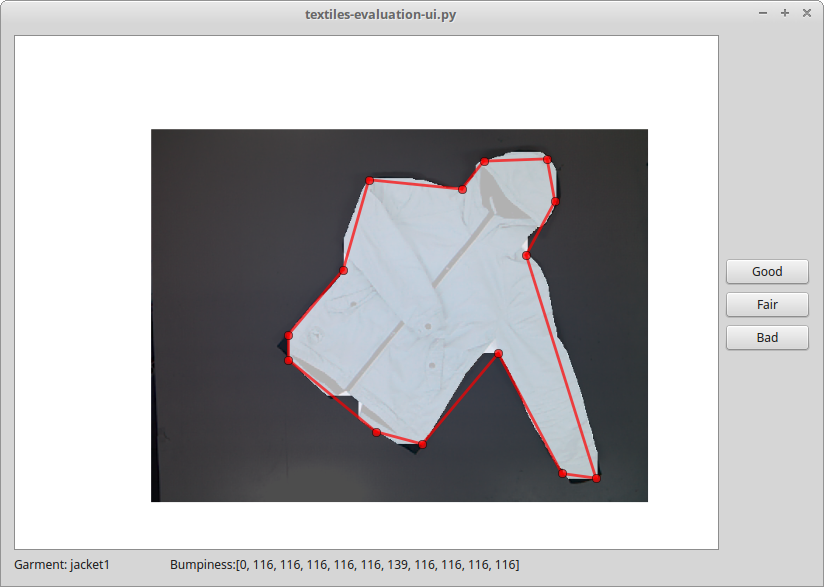
\includegraphics[width=0.7\textwidth]
    {figures/evaluation-gui.png}
    \caption[\comment{GUI}]
    {\comment{GUI}}
    \label{fig:gui}
\end{figure}


Some extra information is also provided in the bottom part of the GUI, such as the name of the garment being evaluated and the bumpiness value for all the candidate unfold paths. Results from each of the 3 stages of our algorithm are first calculated by running the algorithm with all the garment samples. Then, these results are presented consecutively for all the samples in the dataset, and if any of them is evaluated as \fail{}, the remaining ones are skipped for that garment, and automatically evaluated as \discarded{}. All these evaluations are logged and when there are no results left to score, the statistic analysis of the logged evaluations is performed and presented to the evaluator. 

\section{Algorithm Evaluation}
\label{experiments:evaluation}

Previously to testing on the real robot, the algorithm was evaluated using a garment dataset presenting folded garment samples from several different garment categories. These results are later scored with a qualitative metric and then analyzed. This section addresses the garment dataset, the qualitative metric developed and the analysis of these results.

\subsection{Garment Dataset}
\label{experiments:dataset}

To test the computer vision algorithm, a garment dataset was required. A few garment datasets meant for garment manipulation with robots already exist, such as the garment datasets from the CloPeMa project, that have been all made publicly available\footnote{\url{http://clopema.felk.cvut.cz/public_data.html}} to foment algorithm benchmarking. These garment datasets are composed of different types of sensor information (e.g. stereo pairs, depth images, etc) from different kinds of garment samples. There are 4 main datasets, which include samples of spread garments, garments in different stages of a folding sequence and garments being manipulated by a robot arm, both static and in movement. However, after inspection of the samples in these datasets we concluded that they are not suitable to test our algorithm, since these datasets are mainly focused on modeling and folding garments once they are already extended. Our work, nevertheless, is focused on unfolding garments to arrive to the spreaded, unfolded state, so it requires the garments to be flat and present some overlapped regions (folds).

As none of them fit the algorithm developed in this work, a new folded garment dataset was crafted\footnote{\url{http://tinyurl.com/garments-birdsEye-zip}}. The focus of this new dataset is to provide samples of garments placed on a flat surface, and presenting some amount of folds. This pose simulates the result of randomly spreading a garment over a table after picking it from a pile and prior to folding the garment.
To assure some extent of variability within the dataset, the samples were taken from garments belonging to 6 different and representative garment categories: skirt, jacket, pants, polo, robe and hoodie. There is a total of 120 samples of different folds in garments from the mentioned categories.  Each category set is composed by 20 samples, 10 of which present one fold and 10 of which present two folds in the garment. 

This data was obtained using an ASUS Xtion PRO LIVE with RGB and depth channels set at 640x480 resolution. The sensor was placed on top of the working surface providing a bird's eye view over the garment folding environment, with its image plane almost parallel to the working surface. The garments were placed over the surface and folded, and the RGB-D data was then captured for that pose. This procedure was repeated 20 times with different folds for each of the 120 garments that compose the dataset.

\subsection{Experiments}
\label{experiments:experiments}

Using the garment dataset described in the previous section, the algorithm is applied to each of the dataset samples, recording the output at each of the 3 stages of the algorithm. Figures \ref{fig:results}, \ref{fig:results2} and \ref{fig:results3} show the final output of the algorithm and the computed unfolding directions for 4 garments of each of the 6 categories.

\begin{figure}[htbp]
	\centering
	%%%%%%%%%%%%%%%%%%%%%%%%%%%%%%%%%% FigA %%%%%%%%%%%%%%%%%%%%%%%%%%%%%%%%%%%%%%%%%%%%%
	\begin{subfigure}[l]{\bigtablewidth}
	    \centering
    	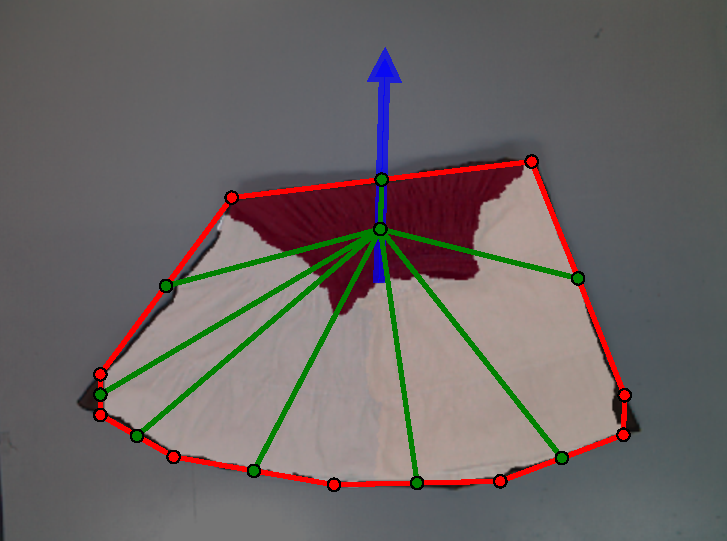
\includegraphics[width=\textwidth]
    	{figures/results/skirt3-pnp.pdf}
	\end{subfigure}
	~
	\begin{subfigure}[r]{\bigtablewidth}
	    \centering
    	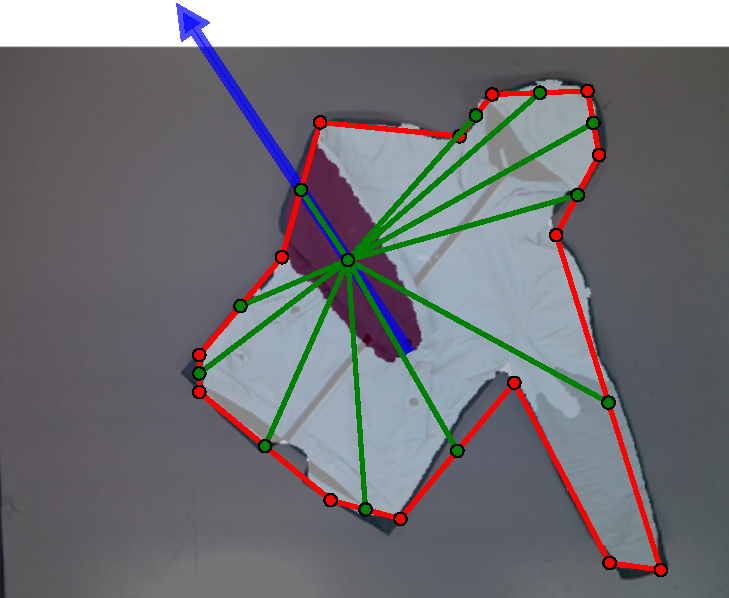
\includegraphics[width=\textwidth]
    	{figures/results/jacket1-pnp.pdf}
	\end{subfigure}
	~
    \begin{subfigure}[l]{\bigtablewidth}
	    \centering
    	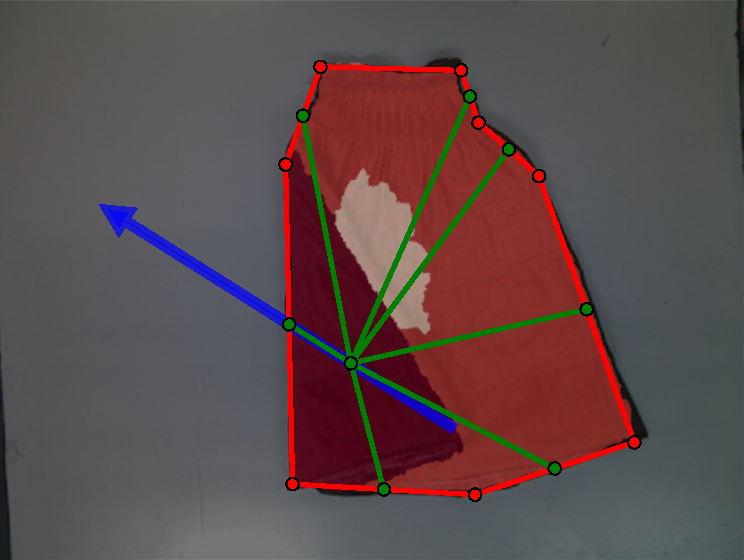
\includegraphics[width=\textwidth]
    	{figures/results/skirt7-pnp.pdf}
	\end{subfigure}
	~
    \begin{subfigure}[r]{\bigtablewidth}
	    \centering
    	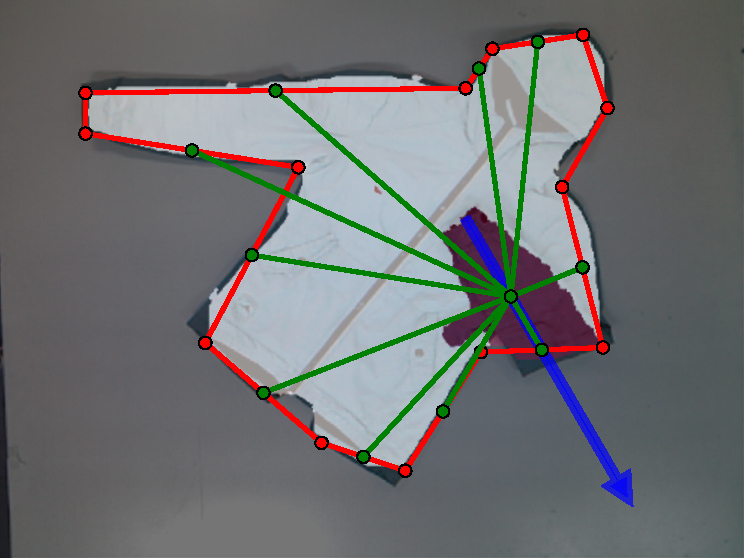
\includegraphics[width=\textwidth]
    	{figures/results/jacket2-pnp.pdf}
	\end{subfigure}
	~
    \begin{subfigure}[l]{\bigtablewidth}
	    \centering
    	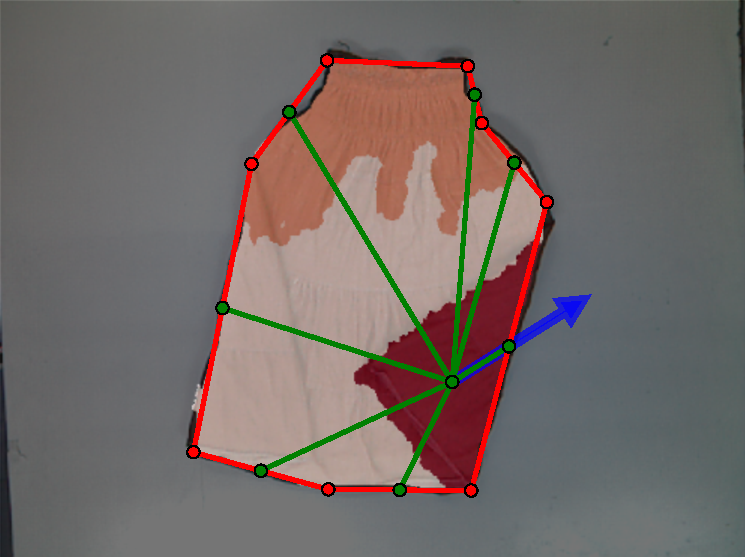
\includegraphics[width=\textwidth]
    	{figures/results/skirt13-pnp.pdf}
	\end{subfigure}
	~
    \begin{subfigure}[r]{\bigtablewidth}
	    \centering
    	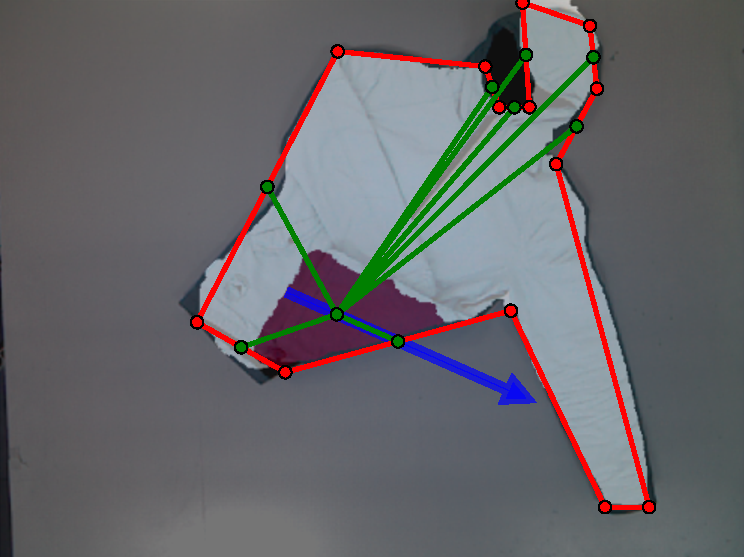
\includegraphics[width=\textwidth]
		{figures/results/jacket12-pnp.pdf}
	\end{subfigure}
	~
    \begin{subfigure}[l]{\bigtablewidth}
	    \centering
    	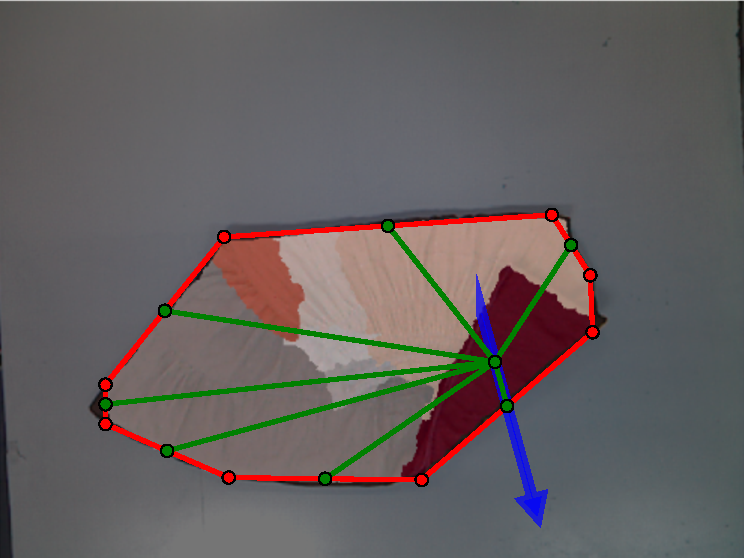
\includegraphics[width=\textwidth]
    	{figures/results/skirt19-pnp.pdf} 
	\end{subfigure}
	~
    \begin{subfigure}[r]{\bigtablewidth}
	    \centering
    	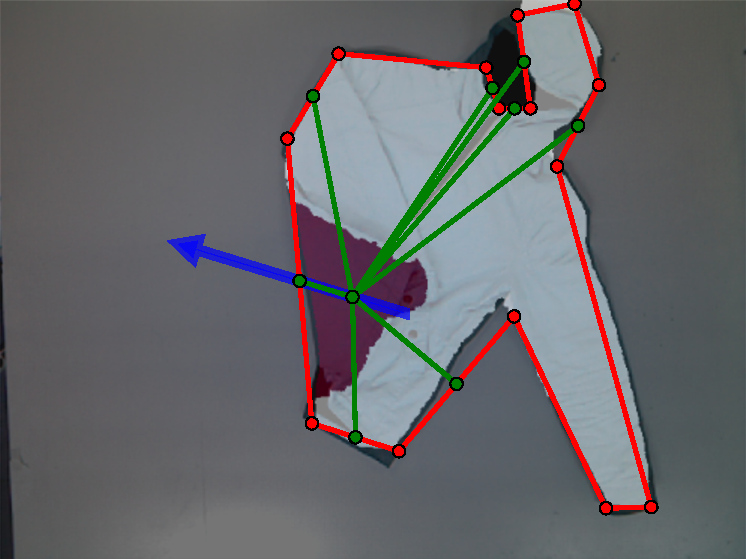
\includegraphics[width=\textwidth]
		{figures/results/jacket13-pnp.pdf}    	
	\end{subfigure}
    \caption[Final output of the algorithm and the computed unfolding directions (Skirt and jacket)]
    {Final output of the algorithm and the computed unfolding directions. Each column includes the output corresponding to 4 of the 20 database samples for each of the 6 garment categories considered. This figure includes the categories Skirt and Jacket.}
    \label{fig:results}
\end{figure}

\begin{figure}[htbp]
	\centering
	%%%%%%%%%%%%%%%%%%%%%%%%%%%%%%%%%% FigB %%%%%%%%%%%%%%%%%%%%%%%%%%%%%%%%%%%%%%%%%%%%%
	\begin{subfigure}[l]{\bigtablewidth}
	    \centering
    	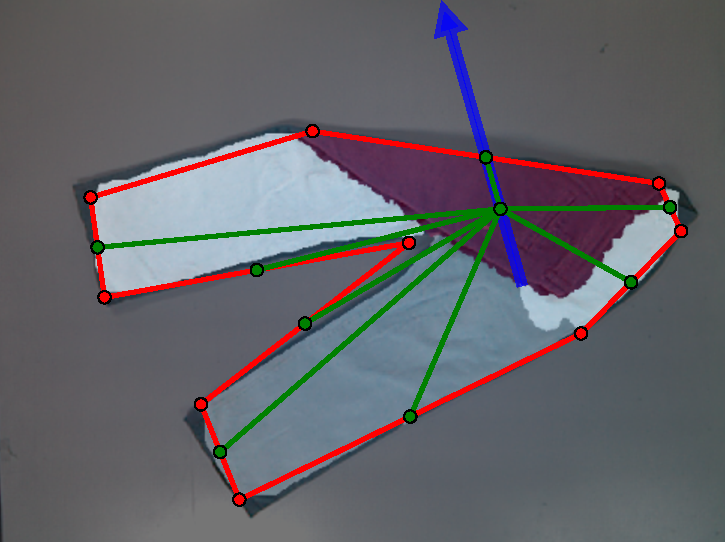
\includegraphics[width=\textwidth]
    	{figures/results/pants7-pnp.pdf}
	\end{subfigure}
	~
	\begin{subfigure}[r]{\bigtablewidth}
	    \centering
    	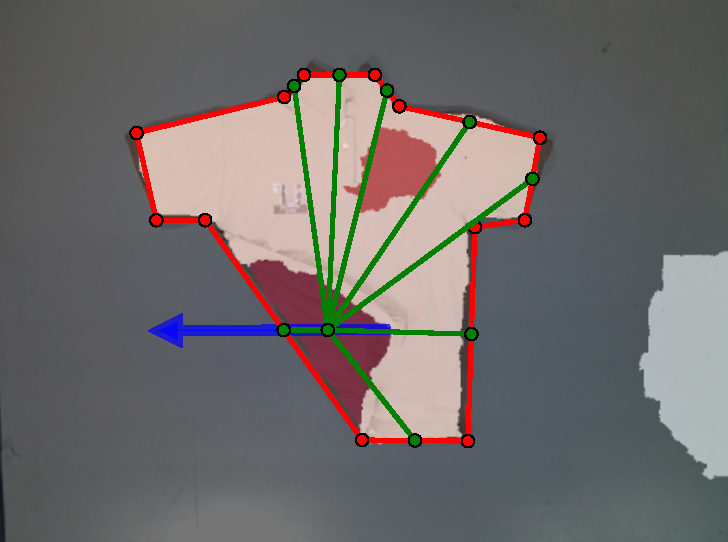
\includegraphics[width=\textwidth]
    	{figures/results/polo1-pnp.pdf}
	\end{subfigure}
	~
    \begin{subfigure}[l]{\bigtablewidth}
	    \centering
    	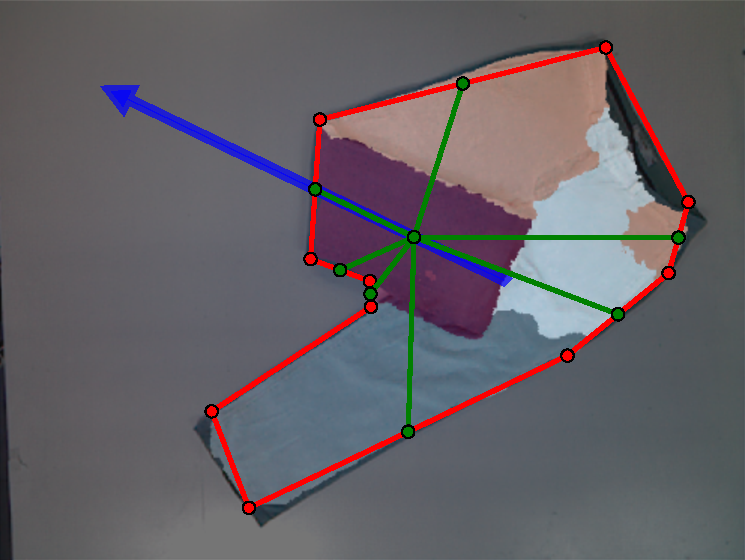
\includegraphics[width=\textwidth]
    	{figures/results/pants8-pnp.pdf}
	\end{subfigure}
	~
    \begin{subfigure}[r]{\bigtablewidth}
	    \centering
    	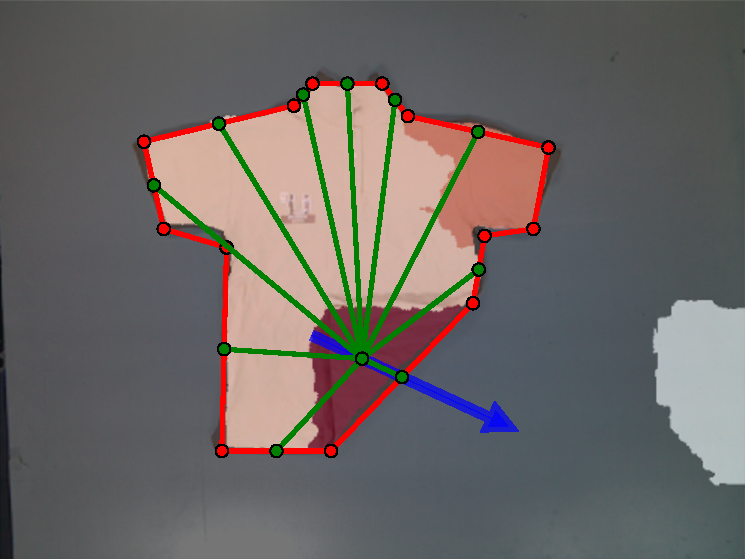
\includegraphics[width=\textwidth]
    	{figures/results/polo2-pnp.pdf}
	\end{subfigure}
	~
    \begin{subfigure}[l]{\bigtablewidth}
	    \centering
    	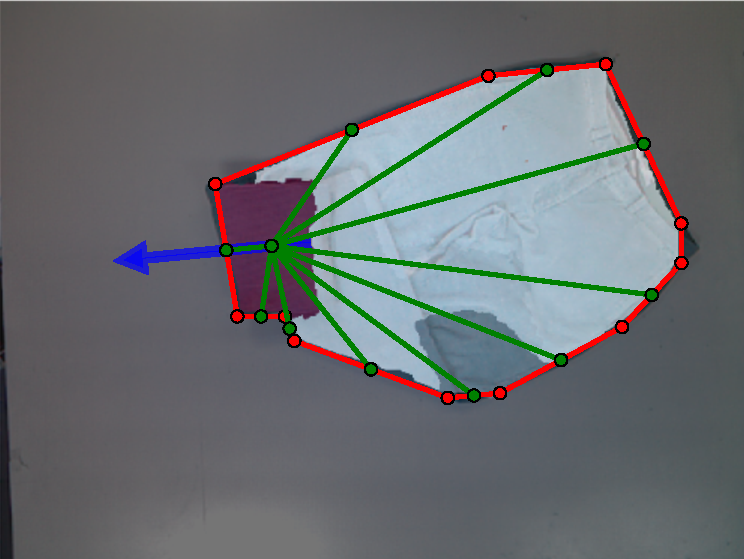
\includegraphics[width=\textwidth]
    	{figures/results/pants14-pnp.pdf}
	\end{subfigure}
	~
    \begin{subfigure}[r]{\bigtablewidth}
	    \centering
    	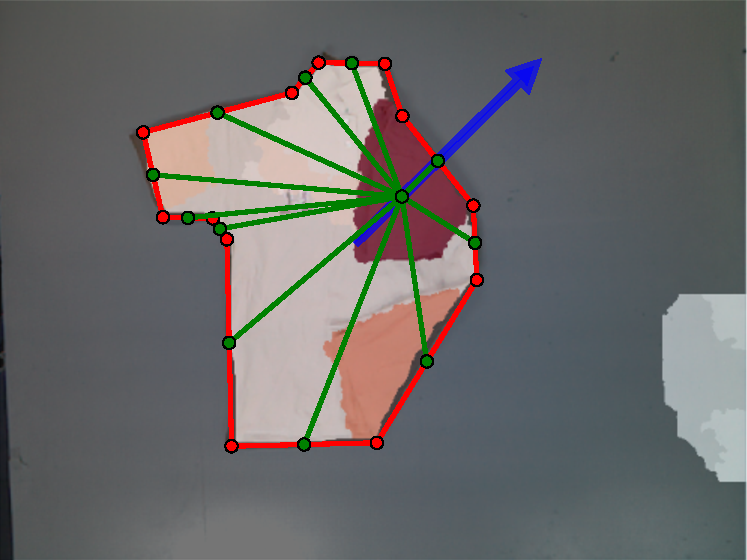
\includegraphics[width=\textwidth]
    	{figures/results/polo13-pnp.pdf}
	\end{subfigure}
	~
    \begin{subfigure}[l]{\bigtablewidth}
	    \centering
    	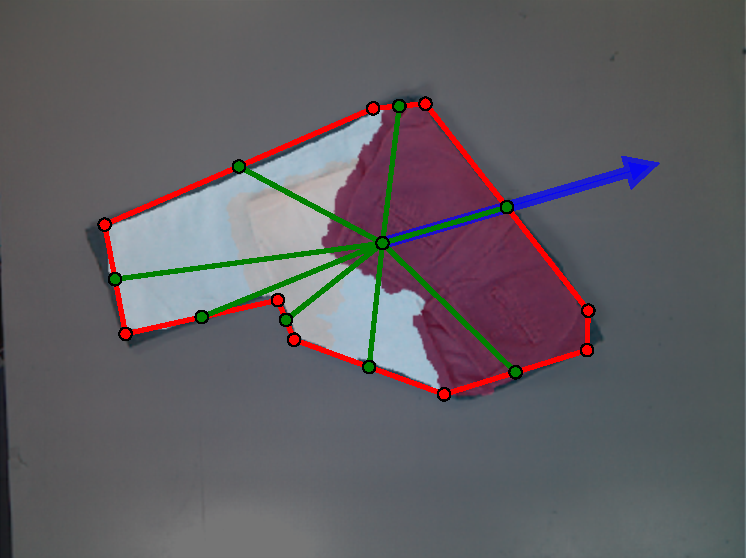
\includegraphics[width=\textwidth]
    	{figures/results/pants15-pnp.pdf}
	\end{subfigure}
	~
    \begin{subfigure}[r]{\bigtablewidth}
	    \centering
    	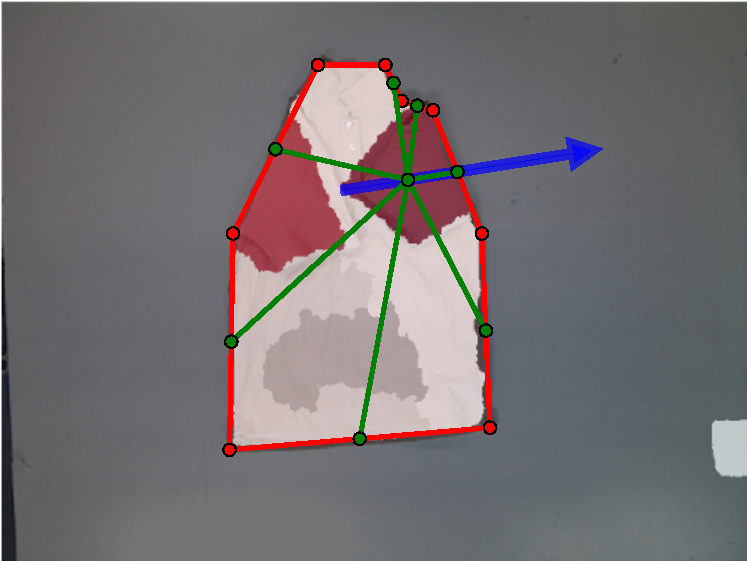
\includegraphics[width=\textwidth]
    	{figures/results/polo15-pnp.pdf}
	\end{subfigure}
	\caption[Final output of the algorithm and the computed unfolding directions (Pants and Polo).]
    {Final output of the algorithm and the computed unfolding directions. Each column includes the output corresponding to 4 of the 20 database samples for each of the 6 garment categories considered.This figure includes the categories Pants and Polo.}
    \label{fig:results2}
\end{figure}

\begin{figure}[htbp]
	\centering
	%%%%%%%%%%%%%%%%%%%%%%%%%%%%%%%%%% FigC %%%%%%%%%%%%%%%%%%%%%%%%%%%%%%%%%%%%%%%%%%%%%
	\begin{subfigure}[l]{\bigtablewidth}
	    \centering
    	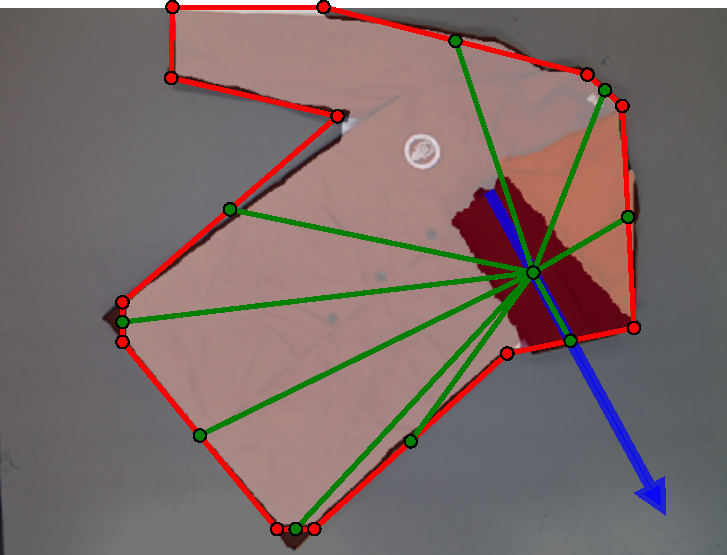
\includegraphics[width=\textwidth]
    	{figures/results/robe4-pnp.pdf}
	\end{subfigure}
	~
    \begin{subfigure}[r]{\bigtablewidth}
	    \centering
    	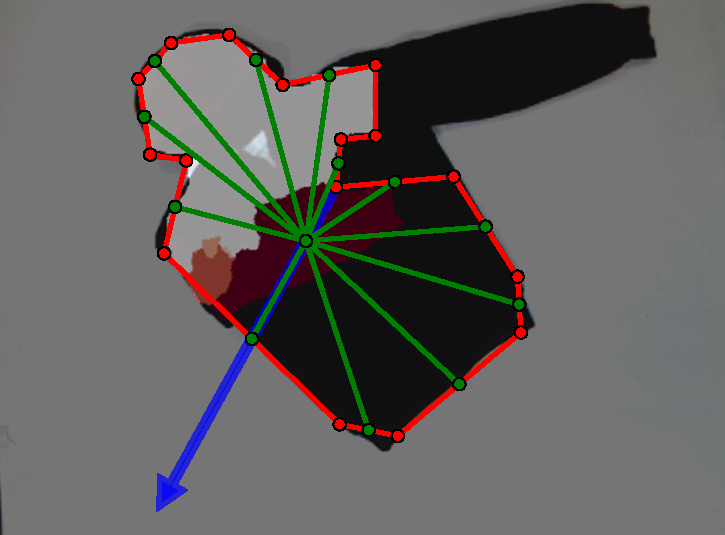
\includegraphics[width=\textwidth]
    	{figures/results/hoodie1-pnp.pdf}
	\end{subfigure}
	~
    \begin{subfigure}[l]{\bigtablewidth}
	    \centering
    	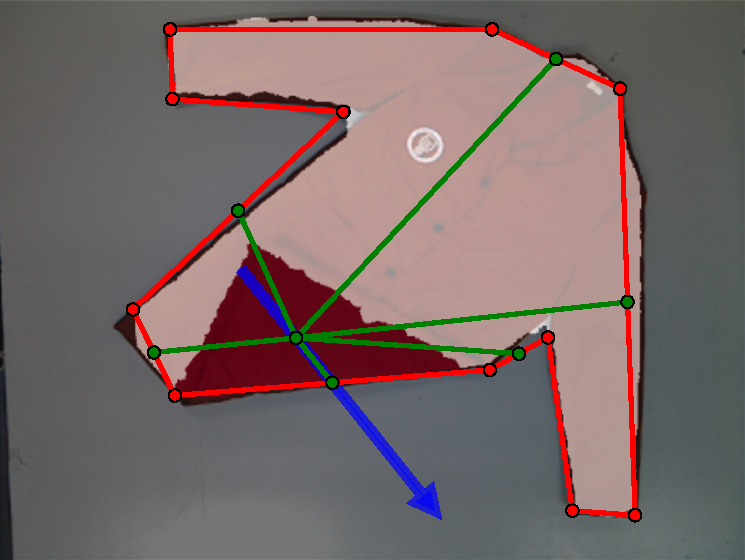
\includegraphics[width=\textwidth]
    	{figures/results/robe8-pnp.pdf}
	\end{subfigure}
	~
    \begin{subfigure}[r]{\bigtablewidth}
	    \centering
    	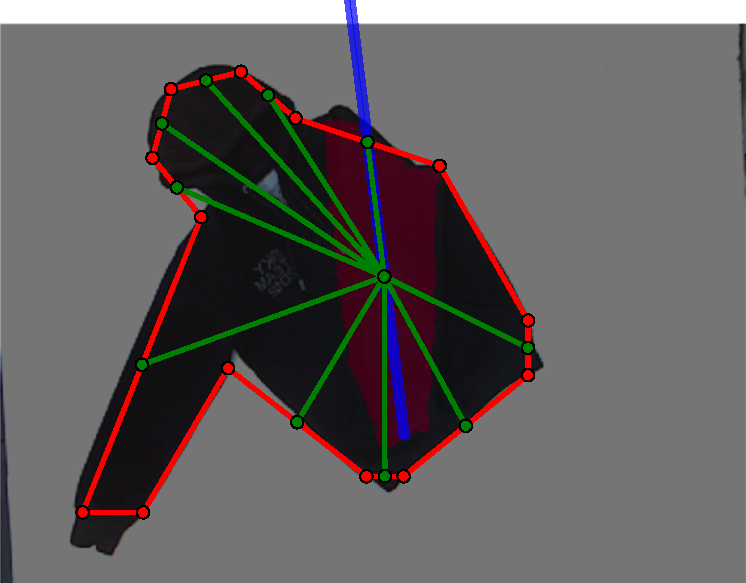
\includegraphics[width=\textwidth]
    	{figures/results/hoodie9-pnp.pdf}
	\end{subfigure} 
	~
	\begin{subfigure}[l]{\bigtablewidth}
	    \centering
    	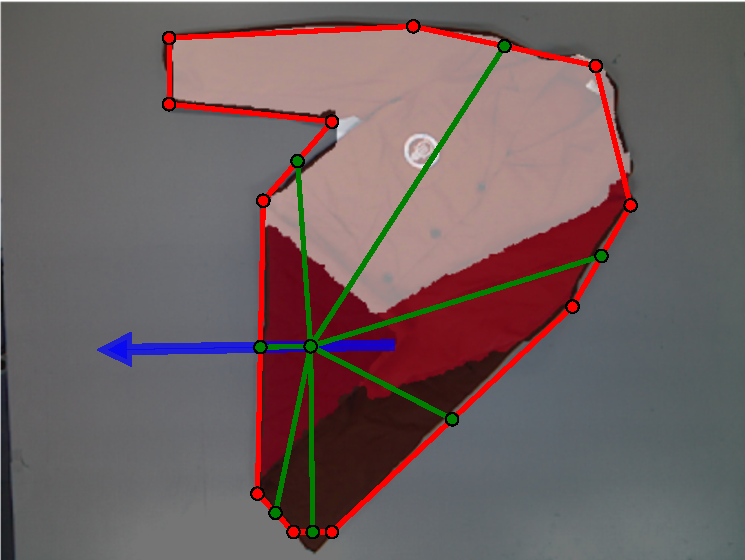
\includegraphics[width=\textwidth]
    	{figures/results/robe15-pnp.pdf}
	\end{subfigure}
	~
    \begin{subfigure}[r]{\bigtablewidth}
	    \centering
    	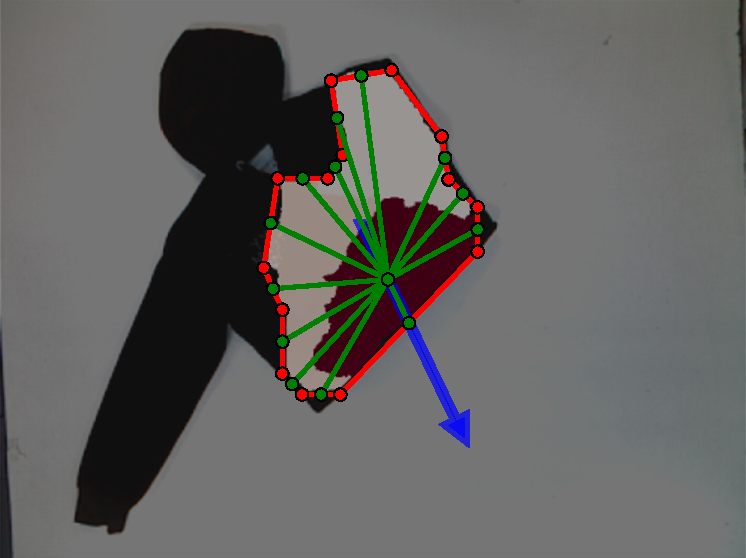
\includegraphics[width=\textwidth]
    	{figures/results/hoodie14-pnp.pdf}    	
	\end{subfigure}
	~
    \begin{subfigure}[l]{\bigtablewidth}
	    \centering
    	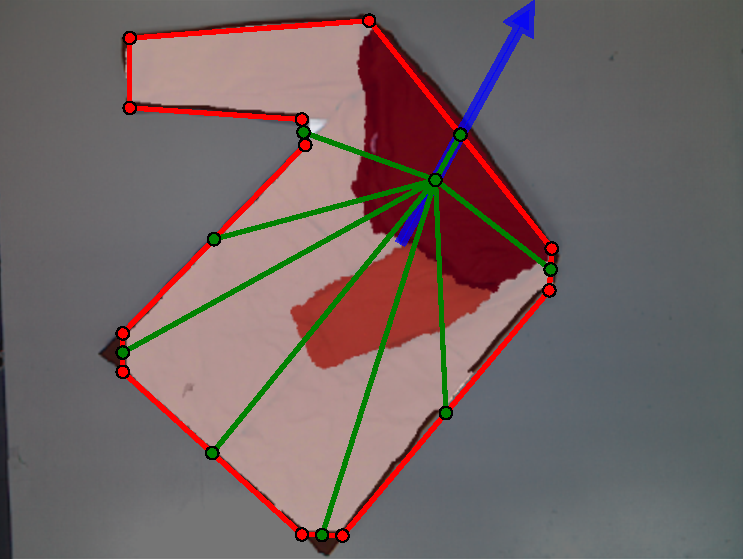
\includegraphics[width=\textwidth]
    	{figures/results/robe19-pnp.pdf}
	\end{subfigure}
	~
    \begin{subfigure}[r]{\bigtablewidth}
	    \centering
    	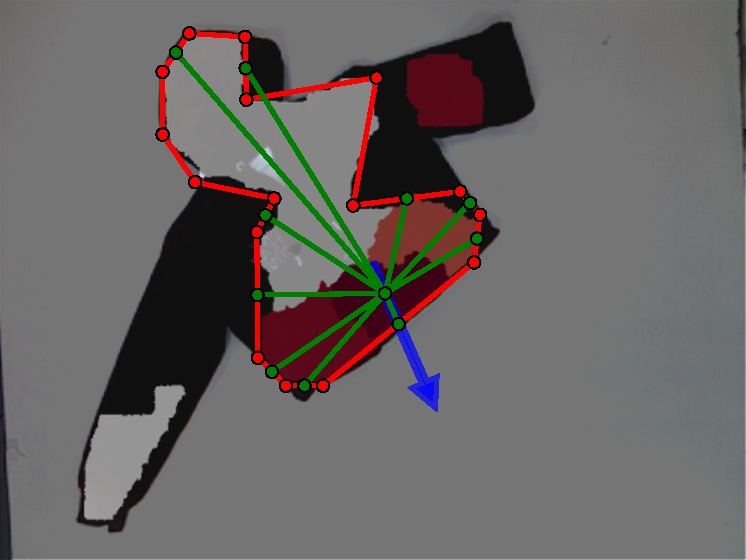
\includegraphics[width=\textwidth]
    	{figures/results/hoodie16-pnp.pdf}
	\end{subfigure} 
    \caption[Final output of the algorithm and the computed unfolding directions (Robe and Hoodie).]
    {Final output of the algorithm and the computed unfolding directions. Each column includes the output corresponding to 4 of the 20 database samples for each of the 6 garment categories considered. This figure includes the categories Robe and Hoodie.}
    \label{fig:results3}
\end{figure}

For evaluating the algorithm, a scoring metric has been established. The criteria for the scoring is qualitative, due to the lack of an objective ground truth to provide quantitative comparisons. The output of each stage is manually classified into one of the following categories: \fail{}, \good{}, \great{} and \discarded{}. Results from one stage that prevent the next one to work properly are classified as \fail{}, and the next stages for that item are classified as \discarded{} and skipped. Results that are not perfect, but allow the next stage to compute its output are classified as \good{}. Note that the \good{} score in the last stage means that the robot could unfold it, but it is not the optimal path. Finally, perfect results for a stage are given the \great{} score.

Table \ref{table:table} shows the raw data of this scoring, indicating the amount of samples that received each score at a given stage for each category.

\begin{table}[htbp]
\centering
\begin{tabular}{|c||c|c c c c|}
\hline 
 & Stage & \fail & \good & \great & \discarded \\ 
\hline \hline
 & Segmentation & 0 & 0 & 20 & 0 \\ 
Skirt & Clustering & 3 & 6 & 11 & 0 \\ 
 & Pick \& Place & 5 & 5 & 7 & 3 \\ 
\hline \hline
 & Segmentation & 0 & 9 & 11 & 0 \\ 
Jacket & Clustering & 8 & 8 & 4 & 0 \\ 
 & Pick \& Place & 3 & 3 & 6 & 8 \\ 
\hline \hline
 & Segmentation & 1 & 1 & 18 & 0 \\ 
Pants & Clustering & 7 & 5 & 7 & 1 \\ 
 & Pick \& Place & 8 & 1 & 3 & 8 \\ 
\hline \hline
 & Segmentation & 0 & 17 & 3 & 0 \\ 
Polo & Clustering & 3 & 13 & 4 & 0 \\ 
 & Pick \& Place & 1 & 4 & 12 & 3 \\ 
\hline \hline
 & Segmentation & 0 & 0 & 20 & 0 \\ 
Robe & Clustering & 5 & 7 & 8 & 0 \\ 
 & Pick \& Place & 3 & 3 & 8 & 6 \\ 
\hline \hline
 & Segmentation & 11 & 3 & 6 & 0 \\ 
Hoodie & Clustering & 6 & 2 & 1 & 11 \\ 
 & Pick \& Place & 3 & 0 & 0 & 17 \\ 
\hline 
\end{tabular} 
\caption{Raw data results of the established scoring metric for each garment category and algorithm stage}
\label{table:table}
\end{table}

Results in each row must add up to 20, since all the garments from each category in the dataset are to be evaluated in each stage. Note also that \fail{} results from previous stages are added to the amount of \discarded{} samples in the last column. The \discarded{} samples have not been presented to the user for evaluation, since previous \fail{} results prevent next stages to yield sucessful results.

A stage by stage analysis is provided in Table \ref{table:table2}. Each cell represents the percent of \good{} and \great{} qualified samples with respect to the amount of samples that actually reached the given stage:

\begin{equation}
cell = \frac{\good + \great}{\fail + \good + \great} \cdot 100 \%
\end{equation}

The Overall performance included in the last row shows the percent of \good{} and \great{} samples taking into account all the samples, including the ones scored as \discarded{}, and corresponds to the product of the percentages of each individual stage, since they are independent events.

\begin{table}[htbp]
\centering
\begin{tabular}{|r||r|r|r|r|r|r||r|}
\hline
	Stage \slash{} Category & Skirt & Jacket & Pants & Polo & Robe & Hoodie & All \\
\hline\hline
   Segmentation         & 100   & 100 &  95   & 100   & 100   & 45   & \textbf{90}\\
   Clustering           &  85   &  60 &  63.2 &  85   &  75   & 33.3 & \textbf{70.4}\\
   Pick \& Place Points &  70.6 &  75 &  33.3 &  94.1 &  78.6 &  0   & \textbf{69.3}\\
   \hline\hline
   Overall              &  60   &  45 &  20   &  80   &    55 &  0   & \textbf{43.3} \\ 
\hline
\end{tabular}
\caption{Results analysis per stage and garment category, expressed in percentage (\%)}
\label{table:table2}
\end{table}

For instance, the Segmentation stage was evaluated as having performed correctly (which includes \good{} and \great{} samples) for 100\% of the Skirt category. With the remaining samples, the Clustering stage performance was evaluated. In this case, within the Skirt category, all of the Skirt samples were evaluated, because they had all passed the previous stage. In this evaluation, 85\% achieved a passing score (\good{} and \great{}). This set of samples was passed on to the Pick \& Place points stage, and for these samples, 70.6\% achieved a passing score within the Skirt category. The Overall algorithm performance for the category is computed as the product of the percentages of three stages: $1 \cdot 0.85 \cdot 0.70 = 60\%$ based on the 20 skirt samples. Table \ref{table:table2} includes an additional column which applies this process based on the evaluation of All the 120 samples of the dataset.


Analyzing the results seen in Table \ref{table:table2}, we can conclude that the Segmentation stage of the algorithm has provided successful results. This stage only achieved low evaluations for the Hoodie, which is black. This might be due to the fact that as this stage relies in color to perform the garment segmentation. As it is using the saturation channel of the HSV color space to detect colorful pixels, and black pixels can have any  saturation value, some pixels may be considered not belonging to the garment. The Clustering stage of the algorithm provides a 70.4\% success rate on the evaluated samples. Certain cluster contours are not fully contained within the region they represent. This may be due to filters used between stages for noise reduction, that may produce a blurring side-effect, and may be adjusted. A fine tuning of Watershed parameters to alter the cluster size could also improve these results. Finally, the Pick and Place Points stage results show our algorithm finds suitable unfolding directions for 69.3\% of the evaluated samples. Regarding the current pick point, the highest garment point or highest region centroid could be used and tested as alternatives. Additionally, instead of using the fold midpoint as a symmetry point to compute the current place point, the entire fold could be used as a symmetry axis for this computation. \comment{However, the success rate of the algorithm, 43.3\%,  improves the current state of the art [in robot unfolding].}

\section{Algorithm Validation}
\label{experiments:validation}

Once the algorithm has been evaluated successfully on the garment dataset, experiments with a real robot were performed to validate the unfolding algorithm. Some clothing articles were provided to the robot over a flat surface, and the robot applied the unfolding algorithm to the input data from the depth sensor to compute the most suitable pick and place points, and then perform an unfolding operation. This section will describe in further detail the experimental setup and the experiments that were executed with the robot.

\subsection{Experimental Setup}
\label{experiments:experimental_setup}

The experimental setup used to perform the evaluation tests consisted of several elements in a laboratory environment: a flat surface, a depth sensor and a humanoid robot. Figure \ref{fig:experimental_setup} depicts this setup.

\begin{figure}[htbp]
    \centering
    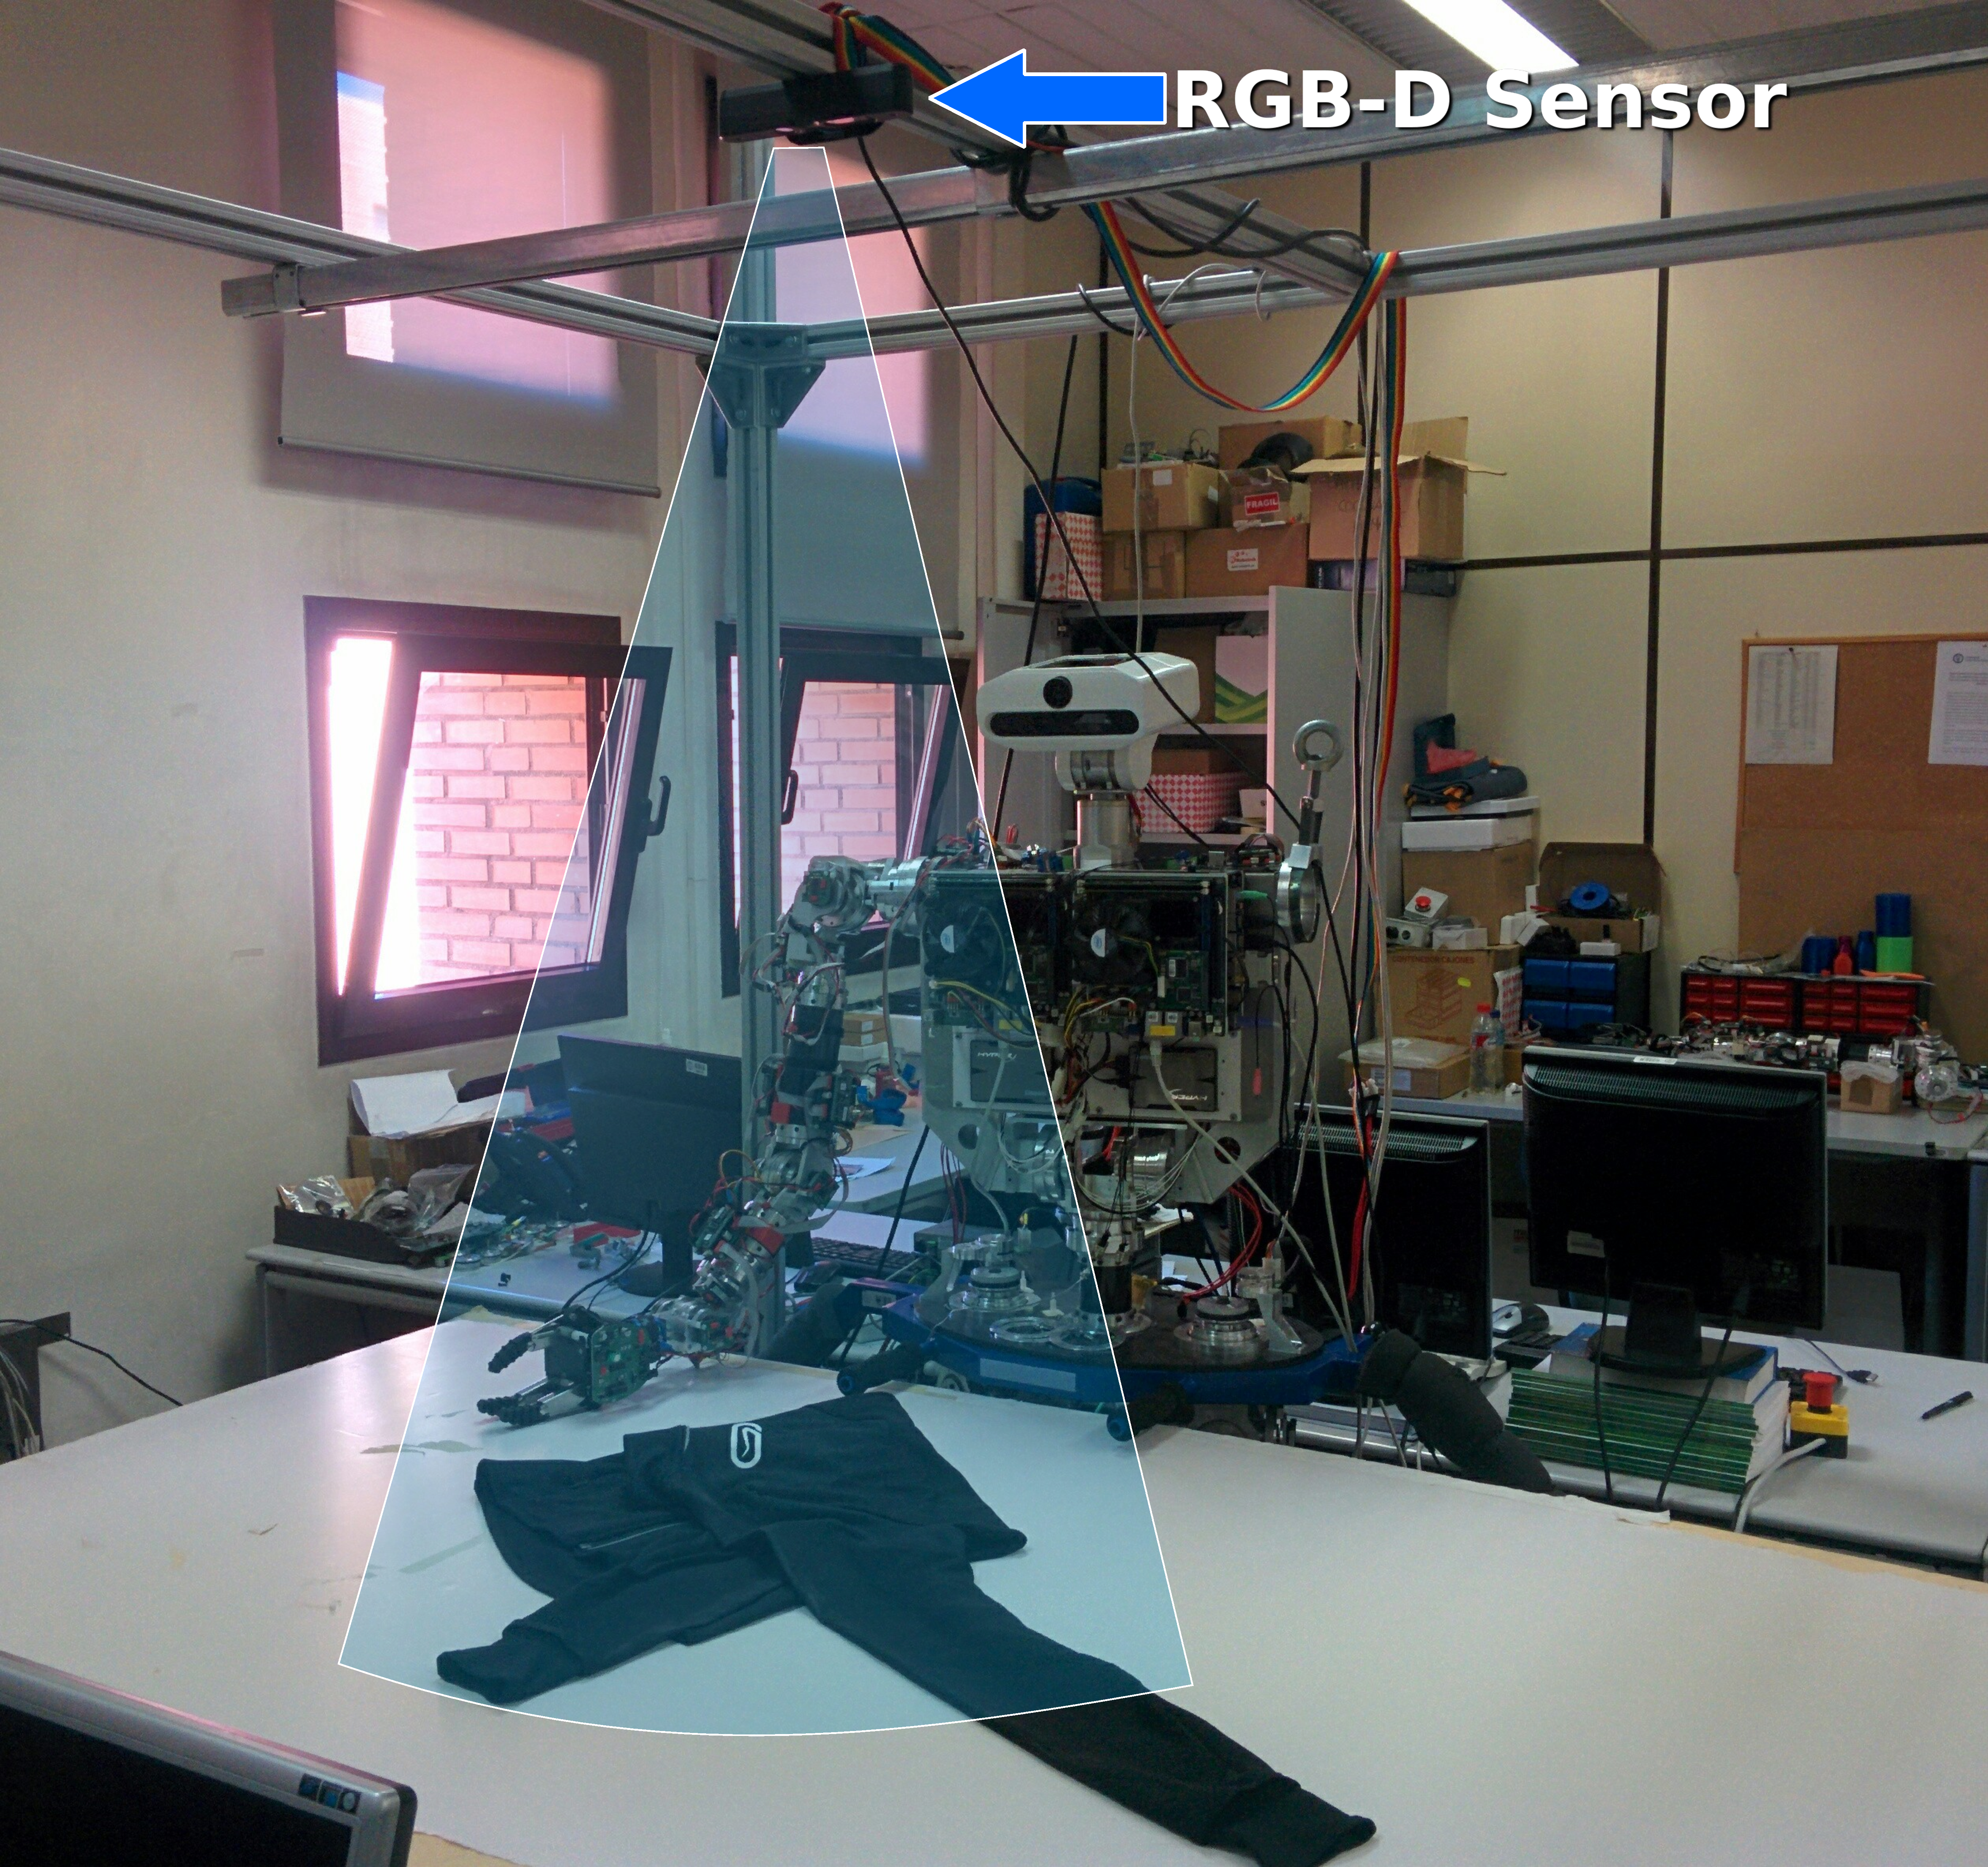
\includegraphics[width=0.8
    \textwidth]{figures/Experimental_setup.pdf}
    \caption[Experimental setup used to test the algorithm]
    {This figure shows the experimental setup used to test the algorithm. The garment rests over a flat white table, with the RGB-D sensor on top. Besides the table, the humanoid robot TEO waits for manipulation trajectories to indicate it how to perform the unfold action.}
    \label{fig:experimental_setup}
\end{figure}

The garment was placed on a white, flat surface, parallel to the floor. Over the garment, an ASUS Xtion PRO LIVE depth sensor was attached to a structure to capture data from a top view, in a position similar to the one used to generate the garment dataset. \comment{Lorem Ipsum goes here, required to make a line break. Come on!}

This final set of laboratory experiments to validate the unfolding algorithm were performed using the full-size humanoid robot TEO \cite{martinez2012teo}. The robot's gripper, designed with passive compliance and relatively large objects in mind (e.g. fruit, bottles, etc), was substituted by a gripper for garment manipulation actuated with hobby servomotors. This gripper was 3D printed in PLA plastic, and controlled with an Arduino board connected by USB to the robot's manipulation computer. 


\subsection{Experiments}
\label{experiments:experiments}
The set of experiments consists in providing several folded garments to the humanoid robot which it has to analyze using the unfolding algorithm presented in this thesis. After the most suitable pick and place points are computed, the humanoid robot should perform and unfolding operation.

The starting point of each experiment is the data adquisition process. The garment data was captured using the ASUS RGB-D sensor in the same configuration (at the ceiling) as for the dataset generation. As garment data is obtained as a point cloud, it needs to be converted to a depth map image for its later analysis. This conversion is done by simply using the z component of each point as the depth value for each pixel of the depth image. If there were a known deviation from the surface (affecting perpendicularity), the depth image could be recovered from the point cloud using the instrinsic and extrinsic parameters of the sensor instead. As the sensor is placed on top of the garment, perpendicular to the surface on which the clothing article rests, both methods yield very similar results, as shown in figure \ref{fig:point_cloud_and_depth_image}.
%- Figure goes here
The RGB values are also recorded for each depth image, obtaining an RGB-D image.

\begin{figure}[htbp]
	\centering
    \begin{subfigure}[l]{0.49\textwidth}
	    \centering
    	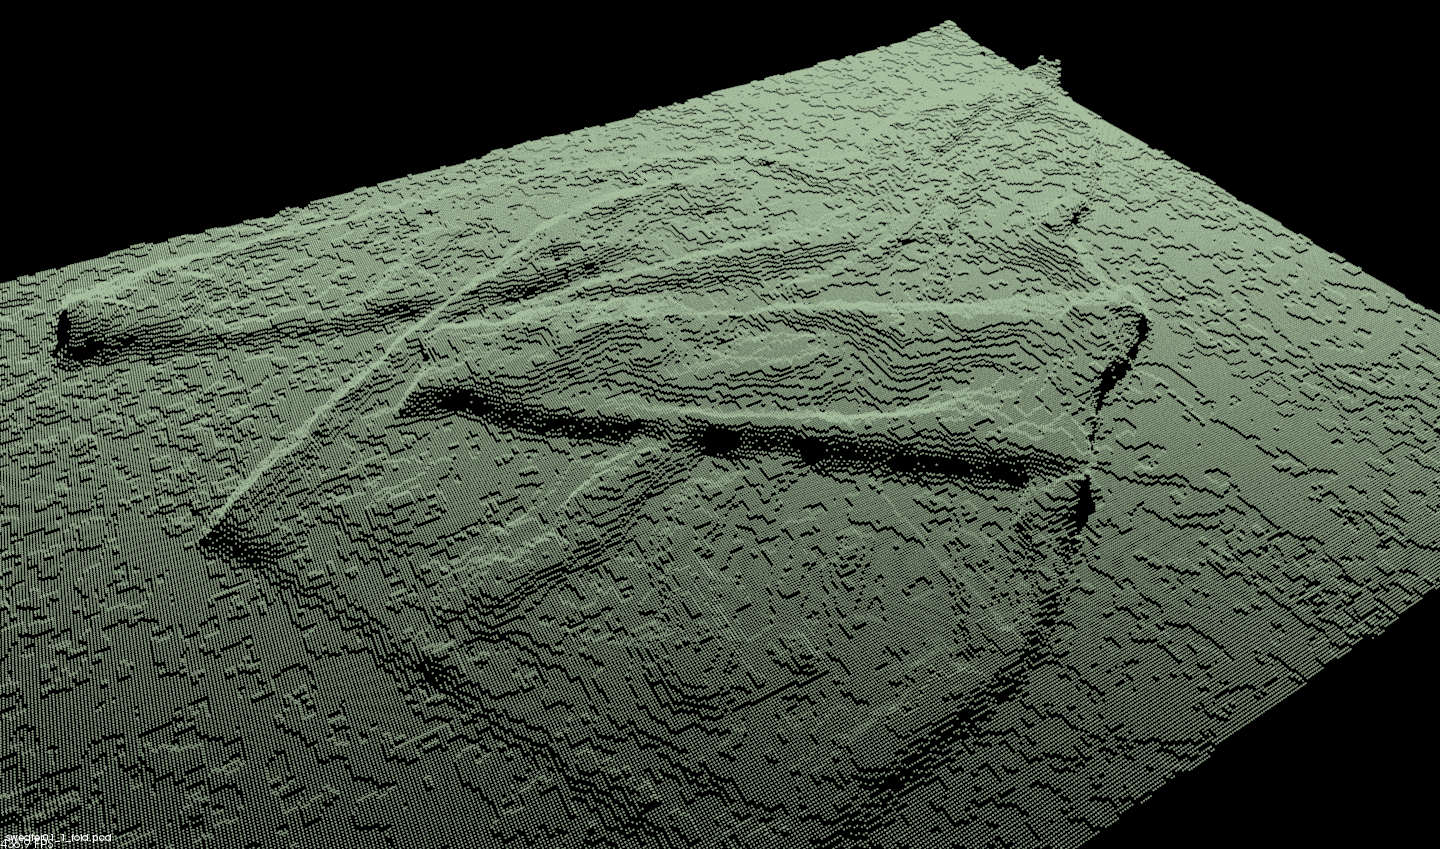
\includegraphics[width=\textwidth]
    	{figures/point-cloud-01.png}
    	\caption{3D Point cloud}
	\end{subfigure}
	~
    \begin{subfigure}[r]{0.49\textwidth}
	    \centering
    	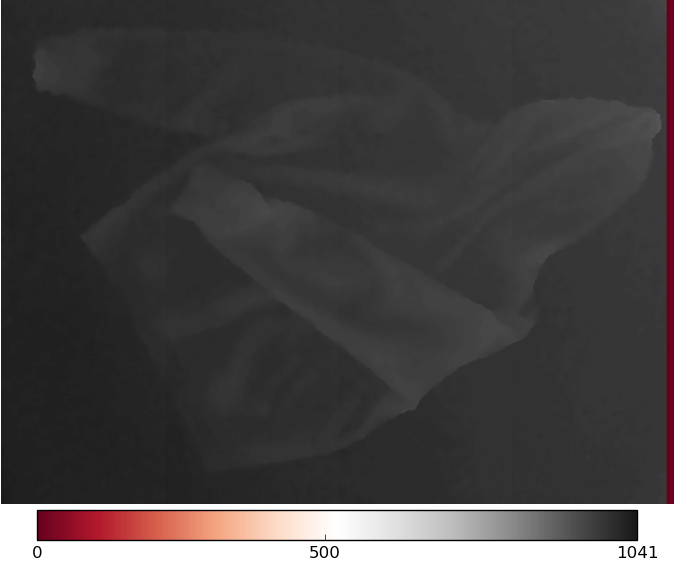
\includegraphics[width=\textwidth]
    	{figures/point-cloud-projection-2.png}
    	\caption{Depth Map}
	\end{subfigure}
    \caption[Comparison of the 3D point cloud with the Depth map obtained from its projection onto the table.]
    {Comparison of the 3D point cloud with the Depth map obtained from its projection onto the table. The colorbar beneath the second figure shows how depth from the camera (in mm) is mapped to the figure colors.}
    \label{fig:point_cloud_and_depth_image}
\end{figure}

Then, the 3 stages of the unfolding algorithm presented in this work are applied consecutively, obtaining the most suitable pick and place points to manipulate the garment. Once the unfolding pick and place points are computed, depth sensor coordinates are converted to the robot root frame. A standard pick and place operation is performed by the robot with the final obtained points.

Figure \ref{} shows the robot performing the unfolding operation.
